\documentclass{beamer}

\usepackage{fancyhdr}
\usepackage[quiet]{fontspec}
\usepackage{tikz}
\usepackage{almslides}
\usepackage{moresize}
\usepackage{hyperref}
\usepackage{svg}
\usepackage{amsmath}

\usetikzlibrary{chains,decorations.pathmorphing,positioning,fit}
\usetikzlibrary{decorations.shapes,calc,backgrounds}
\usetikzlibrary{decorations.text,matrix}
\usetikzlibrary{arrows,shapes.geometric,shapes.symbols,scopes}
\usetikzlibrary{mindmap}

\setmonofont{Monaco}

\title{A Glance at MongoDB}
\author{Sheng Yuan}

\begin{document}
    
\begin{frame}
	\centering
\includegraphics[width=0.7\textwidth]{MongoDB-Logo.png}
    \titlepage
\end{frame}

\begin{frame}{Contents}
    \tableofcontents
\end{frame}

\section{Introduction}
\begin{frame}{Introduction}
	\begin{block}{Document Database}
		A record in MongoDB is a document, which is a data structure composed of field and value pairs. MongoDB documents are similar to JSON objects. 
	\end{block}

	\begin{block}{Tools}
		\begin{Alms*}
			mongo ~~~\    mongoexport ~\ mongooplog ~\ mongos \\
			mongod ~~\    mongofiles ~~\ mongoperf ~~\ mongostat \\
			mongodump     mongoimport ~\ mongorestore  mongotop
		\end{Alms*}
	\end{block}

	\begin{block}{Key Features}
		\begin{itemize}
			\item High Performance
			\item Rich Query Language
			\item High Availability
			\item Horizontal Scalability
			\item Support for Multiple Storage Engines
		\end{itemize}
	\end{block}
\end{frame}

\section{Data Model}
\begin{frame}{Concepts}

\begin{minipage}[t]{0.5\textwidth}
	\scriptsize
	\begin{Alms*}
		\\
		\\
		\\
		> Documents \\
		> Collections \\
		> Database \\
		\\
		\\
		\\
		|\K{Mongodb}~~\ | \K{MySql}~~\ | \\
		|\A {Document}~\ | \A{Row}~~~~\ | \\
		|\A{Field}~~~~\ | \A{Column}~\ | \\
		|\A{Collection}| \A{Table}~~\ | \\
		|\A{Database}~\ | \A{Database}|\\
		|\A{Index}~~~~\ | \A{Index}~~\ |\\
	\end{Alms*}
\end{minipage}
\hfill
\begin{minipage}[t]{0.5\textwidth}
	\scriptsize
	\begin{Alms*}
		> \K{show} \V{dbs} \\
		admin \qquad 0.000GB\\
		local \qquad 0.000GB\\
		firebase \,0.001GB\\
		> \K{use} \V{firebase} \\
		switched to db firebase \\
		> \K{show} \V{collections} \\
		users \\
		models \\
		projects \\
		tasks \\
		> \V{db}.\V{users}.\V{find}().\V{pretty}() \\
		\{ \NI
		"\_id":ObjectId, \\
		"email":"liueh@tcl.com", \\
		"role":"admin"
		\ND \} \\
		\{ \NI
		"\_id":ObjectId, \\
		"email":"yuansheng@tcl.com", \\
		"role":"user"
		\ND \}
	\end{Alms*}
\end{minipage}

\end{frame}

\begin{frame}{Concepts}
	
\end{frame}

\begin{frame}{Data Types}
    \begin{itemize}
        \item Null
        \item Boolean
        \item Integer
        \item Double
        \item String
        \item Date
        \item Array
        \item Embedded Document
        \item ObjectId
        \item BinData
    \end{itemize}
\end{frame}

\section{Working with Data}
\begin{frame}{Mongo Shell}
    The mongo shell is an interactive JavaScript interface to MongoDB. 
    \begin{minipage}[t]{0.5\textwidth}
    	\scriptsize
    	\begin{Alms*}
    		\$ mongo \\
    		MongoDB shell version v3.4.3 \\
    		> \K{show} \V{dbs} \\
    		admin \qquad 0.000GB\\
    		local \qquad 0.000GB\\
    		firebase \,0.001GB\\
    		> \K{use} \V{firebase} \\
    		switched to db firebase \\
    		> \K{show} \V{collections} \\
    		users \\
    		models \\
    		projects \\
    		tasks \\
    		> \V{db}.\V{users}.\V{find}(\{
    		 \NI
    		"email":"liueh@tcl.com"
    		\ND \}).\V{pretty}() \\
    		\{ \NI
    		"\_id":ObjectId, \\
    		"email":"liueh@tcl.com", \\
    		"role":"admin"
    		\ND \}
    	\end{Alms*}
    \end{minipage}
\end{frame}

\begin{frame}{CRUD Operations}
    \begin{minipage}[t]{0.7\textwidth}
        \scriptsize
        \begin{Alms*}
            > db.users.insert(\{"name":"yuansheng"\}) \\
            > db.users.insert(\NI\{"name":"yuansheng", "age":23\}\ND) \\
            > db.users.insert(\NI\{"name":"liueh", "job":"student"\}\ND) \\
            > db.users.find().pretty() \\
            \{ \NI
                "\_id" : ObjectId("58eda18e1d41c860ce59966e"), \\
                "name" : "yuansheng" \\
            \ND \} \\
            \{ \NI
                "\_id" : ObjectId("58eda18e1d41c860ce59966e"), \\
                "name" : "yuansheng" \\
                "age": 23
            \ND \} \\
            > db.users.find(\{"name":"yuansheng"\}).pretty() \\
            > db.users.find(\{"name":"yuansheng"\}).count() \\
            > db.users.find(\{"age":23\}).pretty() \\
        \end{Alms*}
    \end{minipage}
\end{frame}

\begin{frame}{CRUD Operations}
	\begin{minipage}[t]{0.45\textwidth}
		\scriptsize
		\begin{Alms*}
			> db.users.find(\NI
			\{"name":"yuansheng", "age":23\}
			\ND).pretty() \\
			> db.users.find(\{ \NI\$or: [\{age:\{\$gt:18\}\}, \{age:\{\$lt:30\}\}] \ND\})\\
			> db.users.update(\NI
			\{"name":"yuansheng"\},\\
			\{"\$set":\{"name":"yuansheng", "job":"programmer"\}\}
			\ND)
			> db.users.remove(\NI
			\{"name":"yuansheng"\}
			\ND )
		\end{Alms*}
	\end{minipage}
\end{frame}

\begin{frame}{CRUD Operations}
	\begin{minipage}[t]{0.48\textwidth}
		\scriptsize
		\begin{Alms*}
			db.createCollection() \\
			db.collection.drop() \\
			\\
			db.collection.insert() \\
			db.collection.insertOne() \\
			db.collection.insertMany() \\
			\\
			db.collection.find() \\
			db.collection.findOne() \\
			db.collection.findMany() \\
			\\
			db.update()  \\
			db.updateOne() \\
			db.updateMany() \\
			db.collection.replaceOne() \\
			\\
			db.collection.deleteOne() \\
			db.collection.deleteMany() \\
			db.collection.remove()
			
		\end{Alms*}
	\end{minipage}
	\hfill
	\begin{minipage}[t]{0.48\textwidth}
		\scriptsize
		\begin{Alms*}
			db.collection.findAndModify() \\
			db.collection.findOneAndUpdate() \\
			db.collection.findOneAndDelete() \\
			db.collection.findOneAndReplace() \\
		\end{Alms*}
	\end{minipage}
\end{frame}

\section{Advanced Queries}
\begin{frame}{Advanced Queries}
	\scriptsize
	\begin{block}{Specify AND as well as OR Conditions}
		\begin{Alms*}
			db.users.find(\NI \{"name":"yuansheng", "age":23\} \ND) \\
			db.users.find(\NI \{\$or: [\{"name":"yuansheng"\}, \{"age":23\}]\} \ND)
			db.users.find(\NI \{"role":"user", \{\$or: [\{"name":"yuansheng"\}, \{"age":23\}]\}\} \ND)
		\end{Alms*}
	\end{block}

	\begin{block}{Query on Array}
		\begin{Alms*}
			db.users.find(\NI \{tags:\{\$all: ["sports", "read", "travle"]\}\} \ND)
			db.users.find(\NI \{tags: "sports"\} \ND)
			db.users.find(\NI \{steps: \{\$gt: 8000, \$lt: 16000 \}\} \ND)
			db.users.find(\NI \{"steps.1": \{\$gt: 25 \}\} \ND)
			db.users.find(\NI \{steps: \{\$elemMatch: \{\$gt: 8000, \$lt: 16000\}\}\} \ND)
			db.users.find(\NI \{steps: \{\$size: 7 \}\} \ND)
		\end{Alms*}
	\end{block}

\end{frame}

\begin{frame}{Query on Embedded Documents}
	\scriptsize
	\begin{Alms*}
		> db.inventory.insertMany([ \NI
		\{item:"journal", qty:25, size:\{h:14, w:21, uom:"cm"\}, status:"A"\}, \\
		\{item:"notebook", qty:50, size:\{h:8.5, w:11, uom:"in"\}, status:"A"\}, \\
		\{item:"paper", qty:100, size:\{h:8.5, w:11, uom:"in"\}, status:"D"\}, \\
		\{item:"planner", qty:75, size:\{h:22.5, w:30, uom:"cm"\}, status:"D"\}, \\
		\{item:"postcard", qty:45, size:\{h:10, w:15.5, uom:"cm"\}, status:"A"\}
		\ND]);\\
		> db.inventory.find(\{size:\{h: 14, w: 21, uom: "cm"\}\}) \\
		> db.inventory.find(\{"size.uom":"in"\}) \\
		> db.inventory.find(\{"size.h":\{\$lt:15\}\}) \\
		> db.inventory.find(\{"size.h":\{\$lt:15\}, "size.uom":"in", status:"D"\})
	\end{Alms*}
\end{frame}

\begin{frame}{Query an Array of Embedded Documents}
\scriptsize
\begin{Alms*}
	> db.inventory.insertMany([\NI
	\{ item: "journal", instock:[\NI
		\{warehouse: "A", qty: 5\}, \{warehouse: "C", qty: 15\}\ND]\},\\
	\{item: "notebook", instock:[\NI\{warehouse: "C", qty: 5\}\ND]\},\\
	\{item: "paper", instock:[\NI\{warehouse: "A", qty: 60\}, \{ warehouse: "B", qty: 15\}\ND]\},\\
	\{item: "postcard", instock:[\NI\{warehouse: "B", qty: 15\}, \{ warehouse: "C", qty: 35\}\ND]\}
	\ND]);\\
	> db.inventory.find(\{"instock":\{warehouse:"A", qty:5\}\})\\
	> db.inventory.find(\{'instock.0.qty':\{\$lte:20\}\})\\
	> db.inventory.find(\{'instock.qty':\{\$lte:20\}\})\\
	> db.inventory.find(\{"instock":\{\$elemMatch:\{qty:5, warehouse:"A"\}\}\})
\end{Alms*}
\end{frame}

\begin{frame}{Indexs}
	\scriptsize
	\begin{Alms*}
		> db.tasks.find(\NI\{"userid":"liueh@tcl.com"\}
		\ND).limit(1).explain('executionStats') \\
		> db.tasks.find(\NI\{"userid":"liueh@tcl.com"\}
		\ND).explain('executionStats') \\
		\\
		> db.tasks.createIndex({"userid":1}) \\
		> db.tasks.getIndexes() \\
		> db.tasks.find(\NI\{"userid":"liueh@tcl.com"\}
		\ND).explain('executionStats') \\
		\\
		> db.tasks.createIndex({"userid":1, "name":-1}) \\
		> db.tasks.dropIndex() \\
		> db.tasks.dropIndexes()
	\end{Alms*}
\end{frame}

\section{Aggregation}
\begin{frame}{The Aggregation Framework}

\begin{minipage}[t]{0.3\textwidth}
	\begin{Alms*}
	• \$group \\
	• \$limit \\
	• \$match \\
	• \$sort \\
	• \$unwind \\
	• \$project \\
	• \$skip \\
	• \$out \\
	• \$redact \\
	• \$lookup \\
	\end{Alms*}
\end{minipage}
\hfill
\begin{minipage}[t]{0.7\textwidth}
%	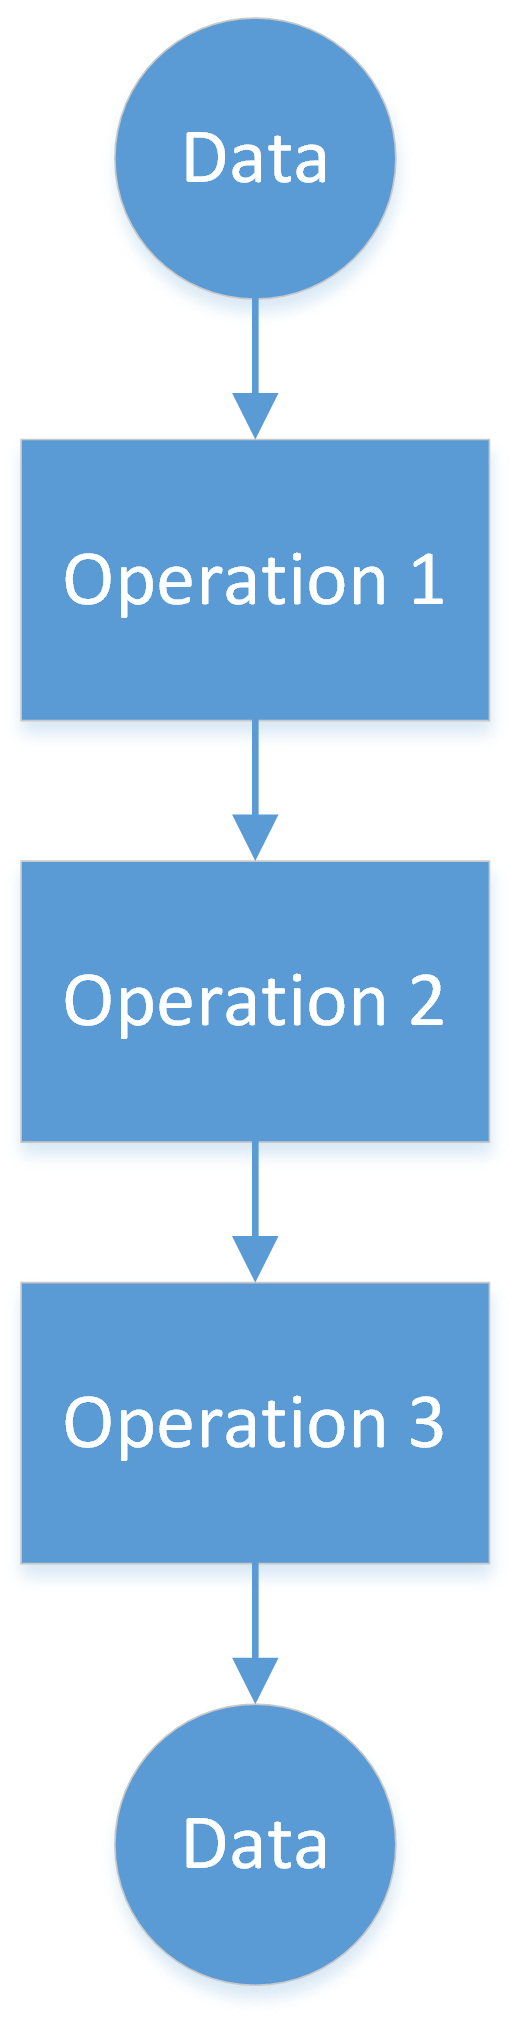
\includegraphics[height=\textheight]{Aggregation-Framework}
%	The aggregation framework in MongoDB represents the ability to perform a selection of matching, grouping,
%	and transformation operations on data in your collection. This is done by creating a pipeline of aggregation
%	operations that will be executed in order, first on the data and then each subsequent operation will be on the
%	results of the previous operation. If you are familiar with the Linux or Unix shell, you will recognize this as
%	forming a shell pipeline of operations.
	
\end{minipage}

\end{frame}

\begin{frame}{The Aggregation Framework}

	\scriptsize
	\begin{Alms*}
	db.users.aggregate(\NI
	\{"\$group":\{"\_id":"\$role", "count":\{"\$sum": 1\}\}\}, \\
	\{"\$sort":\{"count":-1\}\}, \\
	\{"\$limit":2\}
	\ND )
	\end{Alms*}

\end{frame}


\begin{frame}{The Aggregation Framework}

\begin{Alms*}
	• \$group \\
	• \$limit \\
	• \$match \\
	• \$sort \\
	• \$unwind \\
	• \$project \\
	• \$skip \\
	• \$out \\
	• \$redact \\
	• \$lookup \\
\end{Alms*}

\end{frame}


%\section{Python and MongoDB}
%\begin{frame}{Python and MongoDB}
%\scriptsize
%\begin{Alms*}
%	\T{int} \V{udp\_sendmsg}(\T{struct sock *}\V{sk},
%	\T{struct msghdr *}\V{msg}, \textrm{\ldots}) \\
%	\{ \NI
%	\vdots \\
%	\tikzanchor{lock 1}%
%	\only<8->{\highlight<8-9>{\V{lock\_sock}(\V{sk});} \\}%
%	\K{if} \highlight<6-8>{(\V{unlikely}(\V{sk}$→$\V{pending}))} \{ \NI
%	\highlight<5>{
%		\CCOM{Socket is already corked while preparing it} \\
%		\CCOM{\ldots\,which is an evident application bug. --ANK}
%	} \\
%	\only<9->{\highlight<9>{\V{release\_sock}(\V{sk});} \\}%
%	\V{LIMIT\_NETDEBUG}(\V{KERN\_DEBUG} \S{udp cork app bug 2}); \\
%	\highlight<6>{\K{return} -\D{EINVAL};}
%	\ND\} \\[4pt]
%	\tikzanchor{lock 2}%
%	\only<-7>{\highlight<2,7>{\V{lock\_sock}(\V{sk});} \\}%
%	\highlight<3>{%
%		\V{ret} = \V{ip\_append\_data}(\V{sk}, \V{msg}$→$\V{msg\_iov},
%		\V{ulen}, \textrm{\ldots});} \\
%	\vdots \\
%	\highlight<4>{\V{release\_sock}(\V{sk});} \\
%	\K{return} \V{ret};
%	\ND\}
%\end{Alms*}
%\end{frame}

\section{GridFS}
\begin{frame}{GridFS}
	GridFS is a specification for storing and retrieving files that exceed the BSON-document size limit of 16 MB.
	\vspace{0.05\textheight}
	
	\begin{minipage}[t]{0.45\textwidth}
		%
\includegraphics[width=\linewidth]{golang}
		Instead of storing a file in a single document, GridFS divides the file into parts, or chunks, and stores each chunk as a separate document. By default, GridFS uses a chunk size of 255 kB; that is, GridFS divides a file into chunks of 255 kB with the exception of the last chunk.
	\end{minipage}%
	\hfill
	\begin{minipage}[t]{0.45\textwidth}
		\scriptsize
		\begin{Alms*}
		 \$ \K{mongofiles} -d=test \K{list}\\
         \$ \K{mongofiles} \K{put} <filename>\\
         \$ \K{mongofiles} \K{get} <filename>\\
         \$ \K{mongofiles} \K{delete} <filename>\\
         \$ \K{mongofiles} \K{search} <filename>\\
         \$ \K{mongofiles} \K{get\_id} <\_id>\\
         \$ \K{mongofiles} \K{delete\_id} <\_id>\\
		\end{Alms*}
	\end{minipage}
\end{frame}

\begin{frame}{GridFS}
	\begin{minipage}[t]{\textwidth}
		GridFS\cite{Chodorow2013MongoDB} uses two collections to store files. One collection stores the file chunks, and the other stores file metadata.
	\end{minipage}
    
    \begin{block}{fs.files}
        \scriptsize
        \begin{Alms*}
            \{ \NI
                "\_id" : ObjectId("58eda18e1d41c860ce59966e"), \\
                "chunkSize" : 261120, \\
                "uploadDate" : ISODate("2017-04-11T11:15:52.551Z"), \\
                "length" : 237406045, \\
                "md5" : "2166f11cee1bd4b2c31fc429524fdae0", \\
                "filename" : "The.Big.Bang.Theory.S01E01.mkv" \\
            \ND \}
        \end{Alms*}
    \end{block}
    
    \begin{block}{fs.chunks}
        \scriptsize
        \begin{Alms*}
            \{ \NI
            "\_id" : ObjectId("58ecbae81d41c81b3962e857"), \\
            "files\_id" : ObjectId("58ecbae81d41c81b3962e856"), \\
            "n" : 0, \\
            "data" : BinData("...")
            \ND \}
         \end{Alms*}
    \end{block}
    
\end{frame}

\begin{frame}{When to Use GridFS}
    \begin{itemize}
        \item If your filesystem limits the number of files in a directory, you can use GridFS to store as many files as needed.
        \item When you want to access information from portions of large files without having to load whole files into memory, you can use GridFS to recall sections of files.
        \item When you want to keep your files and metadata automatically synced and deployed across a number of systems and facilities, you can use GridFS.
        \item \textcolor{red}{Do not use GridFS if you need to update the content of the entire file atomically. As an alternative you can store multiple versions of each file and specify the current version of the file in the metadata. }
        \item \textcolor{red}{If your files are all smaller the 16 MB BSON Document Size limit, consider storing the file manually within a single document instead of using GridFS.}
    \end{itemize}
\end{frame}

\section{Replication}
\subsection{Why Replication}
\begin{frame}{Why Replication}
    A replica set in MongoDB is a group of mongod processes that maintain the same dataset. With multiple copies of data on different database servers, replication provides a level of fault tolerance against the loss of a single database server.
\end{frame}


\subsection{How Replication Works}
\begin{frame}{Start Replication}
\scriptsize
\begin{Alms*}
	> replicaSet = new ReplSetTest({"nodes":3}) \\
	> replicaSet.startSet() \\
	> replicaSet.initiate() \\
	\\
	> conn1 = new Mongo("localhost:20000") \\
	> primaryDB = conn1.getDB("test") \\
	> primaryDB.isMaster() \\
	> conn2 = new Mongo("localhost:20001") \\
	> secondaryDB = conn2.getDB("firebase") \\
	> secondaryDB.users.find() \\
	> secondaryDB.users.insert(...) \\
	> conn2.setSlaveOk() \\
	> primaryDB.adminCommand(\{"shutdown": 1\}) \\
	
	> replicaSet.stopSet() \\

\end{Alms*}

\end{frame}

\begin{frame}{How Replication Works}

\end{frame}

\subsection{Replica Set Administration}
\begin{frame}{Replica Set Administration}
    \scriptsize
    \begin{Alms*}
    	\$ ssh server-1 \\
    	\$ mongod --replSet spock --fork -f /etc/mongod.conf \\
    	\$ ssh server-2 \\
    	\$ mongod --replSet spock --fork -f /etc/mongod.conf \\
    	\$ ssh server-3 \\
    	\$ mongod --replSet spock --fork -f /etc/mongod.conf \\
    	
    	\$ ssh server-1 \\
    	> config = \{"\_id":"spock", \\
    	"members":[\NI
    	\{"\_id":0, "host":"server-1:27017"\}, \\
    	\{"\_id":1, "host":"server-2:27017"\}, \\
    	\{"\_id":2, "host":"server-3:27017"\}
    	\ND]\} \\
    	> rs.initiate(config) \\
    	> rs.add("server-4:27017") \\
    	> rs.remove("server-4:27017") \\
    	> var config = rs.config() \\
    	> rs.reconfig(config)
    	
    \end{Alms*}
\end{frame}


\section{Database Administration}
\begin{frame}{Backup and Restore}
The MongoDB backup utility is called mongodump; this utility is supplied as part of the standard distribution. And mongo restore is used to restore database from the backup file.

\begin{block}{mongodump}
	\scriptsize
	\begin{Alms*}
		mkdir testmongobackup \\
		cd testmongobackup \\
		mongodump \\
		mongodump -d database \\
		mongodump -d database-c collection \\
	\end{Alms*}
\end{block}

\begin{block}{mongorestore}
	\scriptsize
	\begin{Alms*}
		cd testmongobackup \\
		mongorestore -d database --drop \\
		mongorestore -d database -c collection --drop \\
	\end{Alms*}
\end{block}
\end{frame}

\begin{frame}{Import and Export}
	The mongoimport utility can load data from any of three file formats:
	
	\begin{itemize}
		\item CSV
		\item TSV
		\item JSON
	\end{itemize}
	
	\begin{block}{mongoimport}
		\scriptsize
		\begin{Alms*}
			mongoimport --help \\
			mongoimport -d test -c students --type csv \NI --headerline --file students-csv.dat \ND
			
		\end{Alms*}
	\end{block}

	\begin{block}{mongoexport}
		\scriptsize
		\begin{Alms*}
			monogexport --help \\
			mongoexport -d test -c students -o students.dat \\
			
			mongoexport -d test -c students --csv \NI -f classid,name,age -o students-csv.dat \ND	
		\end{Alms*}
	\end{block}

\end{frame}

\begin{frame}{Protect your Server with  Authentication}
    MongoDB supports a role-based access control authentication model with predefined system roles and user-defined custom roles.
    
    \begin{minipage}[t]{0.64\textwidth}
    	\scriptsize
    	\begin{Alms*}
    		> use admin \\
    		> db.createUser(\{\NI
    		"user":"admin", \\
    		"pwd":"pass", \\
    		"roles":[ \NI
    		\{role:"readWrite", db:"admin"\}, \\
    		\{role:"userAdminAnyDatabase", \\db:"admin"\}
    		\ND]
    		\ND \}) \\
    		\$ mongod --auth \\
    		> use admin \\
    		> show collections \\
    		> db.auth("admin", "pass") \\
    		> db.getUsers() \\
    		> use firebase
    		
    	\end{Alms*}
    \end{minipage}
	\hfill
	\begin{minipage}[t]{0.35\textwidth}
		\scriptsize
		\begin{block}{User Roles}
			\begin{itemize}
				\item read
				\item readWrite
				\item userAdmin
				\item readAnyDatabase
				\item readWriteAnyDatabase
				\item userAdminAnyDatabase
				\item dbAdminAnyDatabase
				\item clusterAdmin
			\end{itemize}
		\end{block}
	\end{minipage}
\end{frame}

\begin{frame}{User Manage}
	\begin{minipage}[t]{0.48\textwidth}
		\begin{block}{User Management Methods}
			\scriptsize
			\begin{Alms*}
				db.auth() \\
				db.createUser()	\\
				db.updateUser()	\\
				db.changeUserPassword()	\\
				db.removeUser()	\\
				db.dropAllUsers() \\
				db.dropUser() \\
				db.grantRolesToUser() \\
				db.revokeRolesFromUser() \\
				db.getUser() \\
				db.getUsers() \\
			\end{Alms*}
		\end{block}
	\end{minipage}
	\hfill
	\begin{minipage}[t]{0.48\textwidth}
		\begin{block}{Role Management Methods}
			\scriptsize
			\begin{Alms*}
				db.createRole()	\\
				db.updateRole()	\\
				db.dropRole() \\
				db.dropAllRoles() \\
				db.grantPrivilegesToRole()	\\
				db.revokePrivilegesFromRole() \\
				db.grantRolesToRole() \\
				db.revokeRolesFromRole() \\
				db.getRole() \\
				db.getRoles() \\
			\end{Alms*}
		\end{block}
	\end{minipage}
\end{frame}

\begin{frame}{Other Tools}
	\begin{block}{Tools}
		\begin{Alms*}
			mongo ~~~\    mongoexport ~\ \T{mongooplog} ~\ \T{mongos} \\
			mongod ~~\    mongofiles ~~\ \T{mongoperf} ~~\ \T{mongostat} \\
			mongodump     mongoimport ~\ mongorestore  \T{mongotop}
		\end{Alms*}
	
	\begin{description}
		\item[mongooplog] Pulls oplog entries from another mongod instance.
		\item[mongos] MongoDB shard process.
		\item[mongoperf] Check disk I/O performance.
		\item[mongostat] Returns counters of database operation. 
		\item[mongotop] Tracks/reports MongoDB read/write activities.
	\end{description}
	\end{block}

\end{frame}

\begin{frame}{References}
	\small
    \bibliography{ref}
    \bibliographystyle{plain}
\end{frame}

\end{document}
